\documentclass[10pt]{article}
\usepackage[margin=0.65in]{geometry}
\usepackage{amsmath,amssymb,booktabs,graphicx,array,longtable,fancyvrb,listings}
\usepackage[hidelinks]{hyperref}
\setlength{\parindent}{0pt}
\setlength{\parskip}{3pt}
\setlength{\emergencystretch}{2em}
\makeatletter
\renewcommand\section{\@startsection{section}{1}{0pt}{1.2ex plus .5ex minus .2ex}{.6ex plus .2ex}{\normalfont\large\bfseries}}
\makeatother
\newcommand{\code}[1]{\nolinkurl{#1}}
\newcommand{\NoMargin}{0.10717}
\newcommand{\YesMargin}{0.11}
\newcommand{\ConceptTrainCount}{8}
\newcommand{\ConceptTestCount}{9}
\newcommand{\ParaphraseDescription}{GPT-6.1-sol generated one paraphrase for each of 100 fixed test sources (25 per dataset/class, seed 15), using the earlier override-paraphrase toy example as inspiration. No detector scores were used to select variants. Automated review judged intent preserved for 100/100, but agreed with only 83/100 publisher labels under the narrower override definition. The disagreements concern original positive examples whose standalone intent is ambiguous, such as a training-date question. Preserve publisher labels; these data do not establish independently verified semantic ground truth.}
\newcommand{\ParaphrasePlanStatus}{Done}
\newcommand{\ParaphrasePlanDate}{Nov. 20}
\newcommand{\GenerationDisclosure}{GPT-6.1-sol generated the 100 paraphrases and supplied automated intent/concept-pair reviews through the author-provided local API. Review prompts and all generated texts/judgments are retained in the data notebook and CSVs.}
\newcommand{\ThresholdDescription}{Frozen threshold: \texttt{0.84093482343069081}; seed-15 LoRA: \texttt{0.317700700270521}; zero-shot: \texttt{0.58654493093490601}. LoRA seeds 16/17 use \texttt{0.29217180259891479}, \texttt{0.40921226293162499}, respectively.}
\newcommand{\RandomReferenceDescription}{Cells with AP at/below its random reference or AUROC at/below 0.5: frozen: \code{deepset\_base64}, \code{safeguard\_base64}, \code{safeguard\_zero\_width}; zero\_shot: \code{deepset\_base64}, \code{deepset\_homoglyph}, \code{deepset\_zero\_width}, \code{safeguard\_homoglyph}, \code{safeguard\_zero\_width}. Obfuscation/tokenization shift and widespread benign false alarms undermine the trained probes; the generic English NLI readout also struggles on this mixed-language task. These are explanations to investigate, not established causes. FPR must be read alongside recall; detecting every injection is not useful resistance if benign prompts are also flagged.}
\newcommand{\DriftDescription}{LoRA mean relative drift ranges from 0.1793 to 0.2369 across datasets/seeds. Point-estimate verdicts follow the stated rule; intervals and seed variation must also be considered. A borderline yes whose interval crosses 0.05 does not establish a stable substantial effect. Positive drift establishes movement relative to the frozen reference, not improved detection.}
\newcommand{\ConceptDescription}{LoRA improves full-pool clean/perturbed cosine for all three conditions and seeds. At 112 pairs, mean cosine over 100 draws is 0.0399 frozen versus 0.3001--0.3036 LoRA for zero-width; $-0.1579$ versus 0.4090--0.5655 for homoglyphs; and 0.0887 versus 0.2340--0.2873 for base64. Every matched LoRA-minus-frozen difference is positive across these draws.}
\newcommand{\FigureFinding}{Selected LoRA changes deepset homoglyph AUROC from 0.7768 to 0.8018 (+0.0250); its practical-rule verdict is no, with uncertainty shown by the intervals.}
\newcommand{\ClaimDescription}{LoRA's gradient updates use only clean training examples, yet its selected model outperforms frozen on Safe-Guard homoglyph and zero-width tests, meeting the practical AUROC improvement rule. Perturbed validation AUROC selects the epoch, but no perturbed examples enter weight fitting. Repeated and larger concept samples show higher clean/perturbed class-direction alignment after LoRA across seeds, with the full-test reference supporting the same pattern. Together with representation drift ($D=0.179$--$0.237$), this supports improved relative stability of the label-associated direction under clean-data adaptation. Similarities remain below 1, and base64 alignment improves without reliable detection; neither complete semantic invariance nor operational robustness is established.}
\newcommand{\ErrorSampleDescription}{The sample contains 10 false positives and 6 false negatives.}
\newcommand{\ErrorFinding}{The sampled false alarms concern legitimate requests after obfuscation. The sampled missed injections provide additional cases for inspecting task and instruction redirection. Check language balance and tokenization before attributing these errors to semantic shortcuts.}
\newcommand{\BaselineReproduction}{Clean AUROC reproduces the midsemester results to four decimals; maximum probability difference is 0.000828, so thresholds are recalibrated on validation rather than assuming bitwise CPU/GPU agreement.}
\newcommand{\TruncationDescription}{At the shared 128-token encoder budget, changed-text truncation counts are base64 145/315; homoglyph 85/315; paraphrase 4/100; zero\_width 116/315. Truncation is therefore part of the measured stress condition, not an isolated semantic perturbation effect.}
\newcommand{\ComputeDescription}{Measured mean per-epoch optimization is $B=0.086$ min, epoch-selection evaluation $V=0.134$ min, and final extraction $E=0.219$ min. The three-seed LoRA rerun and representation caching are complete. For the remaining full fine-tuning baseline, budget 20 epochs and three seeds. Assuming optimization costs eight times the restricted LoRA epoch, allow $480B+60V+3E+4\approx54.1$ L4 minutes, including selection, final extraction and other checks. This planning estimate requires a full fine-tuning timing pilot. API latency and human review are additional wall time.}
\newcommand{\ValidationRolesDescription}{There are 132 selection and 137 calibration rows; the original 1,056 training and 315 test rows are unchanged.}
\newcommand{\SelectedEpochDescription}{All three runs completed 20 epochs. Retained checkpoints: seed 15: epoch 13, seed 16: epoch 17, seed 17: epoch 18.}
\newcommand{\FrozenParaphraseFinding}{Frozen paraphrase AUROC is 0.9856 on deepset and 1.0000 on Safe-Guard. These results concern one generator and do not establish general wording invariance.}

\begin{document}
\begin{center}
{\large\bfseries Understanding Prompt-Injection Detection using LLM-encoded Representations}\\[3pt]
{\bfseries Project 15: Final Checkpoint}\\
Quang Hung Bui \quad COSC 4371, Fall 2026 \quad November 21, 2026\\
\url{https://github.com/hungqbui/security_anaylytics_project}
\end{center}

\fontsize{9}{10.3}\selectfont
\section{Main comparison}
\textbf{Question.} Where does LoRA fine-tuning remain intolerant to intent-preserving perturbations, and what do learned injection-concept representations reveal about these failures? Clean AUROC near 0.99 motivates testing perturbations rather than expecting a meaningful gain at the clean ceiling.

\textbf{(a) Scope change, what ran and what stayed fixed.} To keep the focus simple and accommodate limited compute resources, narrow the planned comparison to four methods: frozen DeBERTa, LoRA, zero-shot NLI, and a standard full fine-tuning baseline. Defer adapters and prompt/prefix tuning. The goal is to examine LoRA's perturbation intolerance through its learned injection-concept representations, including whether adaptation improves ranking while leaving concept separation or benign decisions fragile. This is a question to test, not an assumption that LoRA necessarily reduces robustness.

Completed comparisons use frozen DeBERTa plus a logistic probe (\code{frozen}) and LoRA plus the same probe-fitting protocol (\code{lora}). An auxiliary \code{zero\_shot} detector uses pretrained NLI weights with class descriptions and no prompt-injection training. It is an external control rather than a controlled encoder-adaptation value. Full fine-tuning remains planned; it will use the same data boundaries, pooling and probe evaluation. Score every method on identical rows within each column: clean, zero-width, homoglyph and base64 copies of both datasets, plus the generated-paraphrase subset. Changed copies retain their original IDs and labels. The main checker comparison uses seed 15; seeds 15, 16 and 17 separately assess adaptation stability. They are repetitions, not additional values of the adaptation variable.

Retain the midsemester 1,640 rows: 1,056 training, 269 validation and 315 test rows (116 deepset; 199 Safe-Guard). Use the pinned data/model revisions and exact split construction in the notebooks: seed 15, publisher test partitions, stratified 20\% validation within publisher training, fixed Safe-Guard 800/200 subsamples, and cross-boundary duplicate-group removal. The main encoder is \code{microsoft/deberta-v3-base}, revision \code{8ccc9b6f36199bec6961081d44eb72fb3f7353f3}. Training data, pretrained initialization, 128-token truncation, inference batch 32, last-layer nonspecial/nonpadding mean pooling, test rows and probe hyperparameters remain fixed. No perturbations enter gradient-based weight fitting; they are used for validation selection and testing. Changes since midsemester: replace the one-epoch budget pilot with 20-epoch validation-selected LoRA and perturbation columns; focus concept robustness on clean-versus-perturbed direction similarity within each encoder; use higher AUROC as the direction of interest because the present question concerns improvement. Section 6 gives the reduced remaining plan.

LoRA updates query/value projections in the last two encoder layers: rank 4, scaling 8, dropout 0.05, 24,576 adapter parameters, training batch 8, 20 epochs. A temporary weighted-BCE head supplies the adaptation loss and is discarded. Each final/epoch probe uses training-only StandardScaler and balanced logistic regression ($C=1$, $L_2$, lbfgs, 2,000 iterations). Split original validation rows 50/50 by dataset/label (seed 15), assigning related groups to one role. \ValidationRolesDescription\ Retain the epoch with highest mean selection AUROC across clean/zero-width/homoglyph/base64 copies; clean probe log loss breaks ties. The restored state is scored on test only after selection. Appendix C gives the optimizer details and full learning curves. Runs use Colab NVIDIA L4, Python 3.13.16, with packages in \code{requirements.txt}.

\textbf{Perturbations.} Zero-width inserts U+200B between consecutive ASCII letters. Homoglyph substitution replaces lowercase a/e/o/p/c/x by visually similar Cyrillic letters. Both operate deterministically on every test text, including negatives. Base64 encodes the full UTF-8 request and prepends an instruction to decode and execute it. Its label refers to the decoded request; this is a separate encoding stress test because execution/decoding context and truncation can alter the operative task. \ParaphraseDescription

\textbf{(b) Thresholds.} Positive class 1 is the publisher's injection label; higher scores mean more likely injection. Every detector selects its own threshold on a separate clean calibration subset: the lowest observed score with benign FPR at most 5\%. Reuse that threshold on every changed test column. \ThresholdDescription\ The zero-shot control uses \href{https://huggingface.co/MoritzLaurer/DeBERTa-v3-base-mnli-fever-anli}{Laurer et al. DeBERTa-v3-base NLI model}, revision \code{6f5cf0a2b59cabb106aca4c287eed12e357e90eb}. Pair each text with fixed benign/injection hypotheses and softmax the two entailment logits; the injection probability is the score. Use a 128-token combined premise/hypothesis budget, truncating only the premise, batch 8. Only threshold calibration uses validation labels. Its NLI training and English-language focus differ from the main encoder setup, so this control cannot causally partition dataset and encoder effects.

\textbf{(c) Leakage.} LoRA uses the \emph{same training set}. After duplicate removal, baseline train--test exact-text overlaps and train--validation overlaps are both 0 across pooled datasets; normalized-text, similarity-component and truncated-token overlap checks are also 0. LoRA inherits those same input boundaries. Concept reference pairs use training sources only; held-out concept sources are separate test rows. The zero-shot control fits no encoder or classifier on this project's training labels. These checks explain near-perfect-metric warnings; they cannot exclude unobserved source families, pretraining contamination or lexical shortcuts.

\newpage
\textbf{(d) Primary metric and results.} AUROC is the unchanged primary metric. Intervals are the final checker's 1,000-resample, row-bootstrap 95\% intervals; a column has one variant per source row. LoRA and zero-shot cells use their own thresholds, but AUROC itself is threshold independent. Paraphrase subsets have 25 positives/25 negatives per dataset when present; full deepset has 60/116 positives (51.72\%), Safe-Guard 63/199 (31.66\%). The 25 examples per class in each paraphrase column limit interval precision and power.
\begin{center}\resizebox{\linewidth}{!}{\begin{tabular}{lccccc}
\toprule
\multicolumn{6}{l}{\textbf{deepset}}\\
Method & Clean & Zero-width & Homoglyph & Base64 & Paraphrase\\\midrule
Frozen probe & \textbf{0.9917} [0.9781, 0.9994] & \textbf{0.7673} [0.6650, 0.8535] & \underline{0.7768} [0.6878, 0.8569] & \underline{0.4762} [0.3688, 0.5831] & \underline{0.9856} [0.9566, 1.0000]\\
LoRA (seed 15) & \underline{0.9887} [0.9730, 0.9988] & \underline{0.7399} [0.6445, 0.8247] & \textbf{0.8018} [0.7198, 0.8738] & \textbf{0.5003} [0.3905, 0.6066] & \textbf{0.9920} [0.9708, 1.0000]\\
Zero-shot NLI & 0.6128 [0.5033, 0.7167] & 0.3878 [0.2775, 0.5012] & 0.4667 [0.3524, 0.5771] & 0.4363 [0.3381, 0.5448] & 0.5584 [0.3889, 0.7264]\\
Full fine-tuning & -- & -- & -- & -- & --\\
\midrule
\multicolumn{6}{l}{\textbf{safeguard}}\\
Method & Clean & Zero-width & Homoglyph & Base64 & Paraphrase\\\midrule
Frozen probe & \textbf{0.9956} [0.9892, 1.0000] & \underline{0.4700} [0.3940, 0.5527] & \underline{0.5431} [0.4578, 0.6257] & 0.4972 [0.4088, 0.5789] & \textbf{1.0000} [1.0000, 1.0000]\\
LoRA (seed 15) & \underline{0.9951} [0.9872, 0.9997] & \textbf{0.5993} [0.5187, 0.6809] & \textbf{0.7816} [0.7174, 0.8458] & \underline{0.5180} [0.4347, 0.5996] & \textbf{1.0000} [1.0000, 1.0000]\\
Zero-shot NLI & 0.7870 [0.7014, 0.8673] & 0.2498 [0.1861, 0.3171] & 0.4973 [0.4162, 0.5806] & \textbf{0.5487} [0.4594, 0.6331] & \underline{0.6352} [0.4623, 0.7884]\\
Full fine-tuning & -- & -- & -- & -- & --\\
\bottomrule\end{tabular}
}\end{center}
Bold marks the best AUROC per column; underlining marks the next distinct score. Ties share a rank.
\RandomReferenceDescription\ Score direction was checked: logistic probability column 1 corresponds to label 1; NLI entailment logits follow the configured label map and the injection hypothesis is candidate 1. Scores were not inverted using test outcomes. \FrozenParaphraseFinding

\textbf{(e) Decision rule and verdicts.} The midsemester clean rule was an absolute AUROC change of at least 0.02 for yes, at most 0.00981 for no, intermediate changes inconclusive. Clean gains of 0.02 are impossible at the observed ceiling. As proposed at midsemester, retain a perturbation rule derived solely from frozen results and fixed for this 20-epoch comparison: the widest baseline half-interval across the six zero-width/homoglyph/base64 columns is \NoMargin. A higher-AUROC change $\geq\YesMargin$ is yes; a change $\leq\NoMargin$ is no; intermediate changes are undecided. Changes in the wrong direction are no. These are practical decision thresholds, not significance tests. Apply this fixed rule to paraphrases as a subsequent evaluation without retuning it. The checker changes and verdicts are:
\begin{center}\small\begin{tabular}{lll}
\toprule
Column & LoRA change (verdict) & Zero-shot change (verdict)\\
\midrule
deepset\_base64 & +0.0241 (no) & -0.0399 (no)\\
deepset\_clean & -0.0030 (no) & -0.3789 (no)\\
deepset\_homoglyph & +0.0250 (no) & -0.3101 (no)\\
deepset\_paraphrase & +0.0064 (no) & -0.4272 (no)\\
deepset\_zero\_width & -0.0274 (no) & -0.3795 (no)\\
safeguard\_base64 & +0.0208 (no) & +0.0515 (no)\\
safeguard\_clean & -0.0005 (no) & -0.2086 (no)\\
safeguard\_homoglyph & +0.2386 (yes) & -0.0458 (no)\\
safeguard\_paraphrase & +0.0000 (no) & -0.3648 (no)\\
safeguard\_zero\_width & +0.1293 (yes) & -0.2202 (no)\\
\bottomrule\end{tabular}
\end{center}

\textbf{Stability across seeds.} The table reports AUROC mean, sample SD and range over three runs; the main checker table remains seed 15 rather than pooling repeated predictions as independent test rows. Frozen lbfgs probing is effectively deterministic with these settings, so its zero seed spread is not evidence about variation across datasets. Three LoRA seeds are descriptive and insufficient for strong population-level claims.
The full per-column seed table is in Appendix B.

\newpage
\textbf{Assigned representation-change result.} For matched original test texts $S$, report
\[
 D_m(S)=\frac1{|S|}\sum_{x\in S}\frac{\|h_m(x)-h_0(x)\|_2}{\|h_0(x)\|_2+10^{-12}}.
\]
Frozen self-drift is exactly 0. Use a separate exploratory practical rule: $D\geq0.05$ indicates substantial movement (yes), $D\leq0.01$ indicates small movement (no), otherwise undecided. These thresholds express 5\%/1\% relative representation movement; they are not a robustness criterion or an empirically calibrated cutoff. The 5\%/1\% cutoffs are illustrative practical choices, not preregistered thresholds. Each seed's interval resamples test rows 1,000 times (seed 15); seed spread is reported separately.
\begin{center}\small\begin{tabular}{lrll}
\toprule
Dataset & Seed & $D$ [95\% interval] & Drift verdict\\
\midrule
deepset & 15 & 0.1835 [0.1674, 0.2001] & yes\\
safeguard & 15 & 0.1793 [0.1684, 0.1901] & yes\\
deepset & 16 & 0.2191 [0.1981, 0.2407] & yes\\
safeguard & 16 & 0.2073 [0.1934, 0.2211] & yes\\
deepset & 17 & 0.2369 [0.2106, 0.2658] & yes\\
safeguard & 17 & 0.2074 [0.1906, 0.2241] & yes\\
\bottomrule\end{tabular}
\end{center}
\DriftDescription

\textbf{Concept-direction robustness (change from midsemester).} Estimate a broad publisher-label injection direction from random test injections and benign prompts. Each subset contains $K$ distinct examples per class, equally divided between datasets; no score-based or semantic acceptance filter is applied. The initial 20-pair draw is followed by a sensitivity study at $K=10,20,40,60,80,100,112$, with 100 nested random draws per size (seeds 17--116). The same source subsets are used across models and conditions. These are post-hoc representation diagnostics; they never choose weights, epochs or thresholds.
\[
 v_m^{\rm clean}(K)=\frac1K\sum_{j=1}^K[h_m(I_j)-h_m(B_j)],\qquad
 v_m^T(K)=\frac1K\sum_{j=1}^K[h_m(TI_j)-h_m(TB_j)],
\]
\[
 R_m(T;K)=\frac{(v_m^{\rm clean}(K))^\top v_m^T(K)}
 {\|v_m^{\rm clean}(K)\|_2\|v_m^T(K)\|_2}.
\]
Near 1 means a stable class-contrast direction. Pairing order does not affect the difference of class means; averaging reduces sampling variation but cannot remove systematic label/topic confounding. Samples use equal dataset weights. The largest balanced size is 112 pairs, limited by the 56 deepset benign rows. For a full-pool reference, use all 315 test prompts with the same equal-dataset target:
\[
 v_{m,\mathrm{all}}^{s}=\frac12\sum_{d\in\{\mathrm{deepset},\mathrm{safeguard}\}}
 (\bar h_{m,d,1}^{s}-\bar h_{m,d,0}^{s}),
\]
where each $\bar h$ is the class mean within its dataset and condition $s$. The full-pool clean/perturbed cosines are:
\begin{center}\small\begin{tabular}{lrlll}
\toprule
Method & Seed & Zero-width & Homoglyph & Base64\\\midrule
frozen & 15 & 0.0297 & -0.1873 & 0.0893\\
lora & 15 & 0.2976 & 0.4036 & 0.2393\\
lora & 16 & 0.3026 & 0.5629 & 0.2872\\
lora & 17 & 0.2989 & 0.5630 & 0.2339\\
\bottomrule\end{tabular}
\end{center}
\ConceptDescription\ At $K=112$, subset directions approach their full-pool references (mean cosine at least 0.971 across conditions/models), while clean/perturbed alignment remains below 1. Thus larger samples support relative alignment improvement, not complete invariance. Appendix E gives the sample-size curves and spreads; these characterize this fixed pool, not independent-dataset confidence intervals. The initial 20-pair result and bootstrap intervals remain in Appendix D.

The mean-difference construction is related to \href{https://aclanthology.org/2024.acl-long.828/}{contrastive activation addition (Rimsky et al., 2024)}; original \href{https://proceedings.mlr.press/v80/kim18d/kim18d.pdf}{TCAV (Kim et al., 2018)} learns a classifier normal. The earlier screened-pair gap diagnostics use a narrower override concept (Appendix D).

\newpage
\section{Figure}
\begin{center}
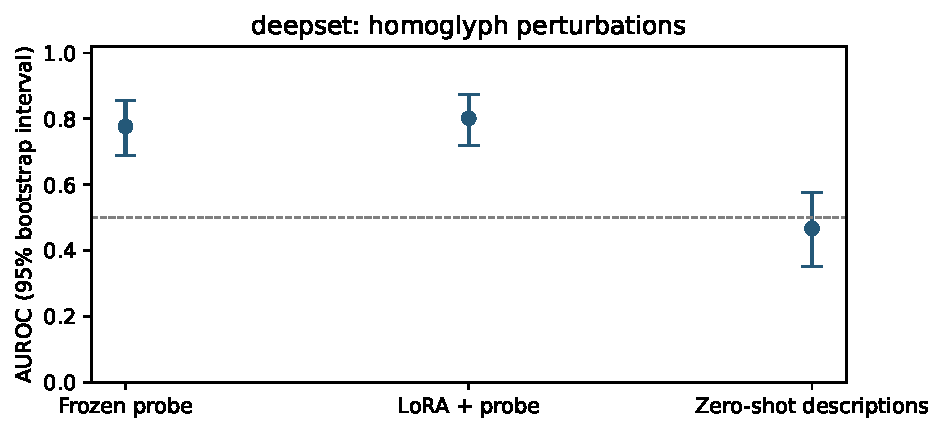
\includegraphics[width=.74\linewidth]{final_comparison.pdf}\\
\small Figure 1. AUROC with checker-matched 95\% intervals for \code{deepset\_homoglyph}: 116 test rows, 60 positive (51.72\%). Values: frozen probe, seed-15 LoRA probe, and zero-shot descriptions.
\end{center}
\FigureFinding

\section{Claim and limitation}
\textbf{(a) Claim.} \ClaimDescription

\textbf{(b) Limitation.} The AUROC gains do not establish reliable detection at the clean-calibrated threshold: Safe-Guard homoglyph FPR rises from 0.5956 to 0.7868, and zero-width FPR remains 1.0000. Thus the positive verdicts concern ranking improvement; threshold transfer and benign false alarms remain unresolved.

\textbf{Interpretation and next check.} The original single 20-pair draw is atypical: its mixed changes do not represent the larger repeated-sampling result. With more examples, the mean class directions stabilize and LoRA retains greater clean/perturbed alignment than frozen on this pool. This supports improved class-direction stability alongside Safe-Guard ranking gains, while base64 remains a counterexample to treating alignment alone as detector robustness. Label ambiguity, topic effects, dataset-specific behavior and threshold transfer remain unresolved. Appendix C relates validation drift to AUROC; the remaining method comparison is full fine-tuning.

\section{Error analysis}
\textbf{(a) Sample.} From \code{frozen / deepset\_homoglyph}, sample 10 false positives and 10 false negatives at random (seed 15), taking all errors of a type when fewer than 10 exist. \ErrorSampleDescription\ Every sampled row appears once in \code{errors.csv}; \code{error\_examples.csv} includes its text and score.

\textbf{(b) Categories.} Categories describe source content rather than proving a causal failure mechanism. Categorize from the original unobfuscated text. ``German benign request'' is a false alarm whose source contains a German cue (wie, wieviele, was, mein, ich, der, kinder, deutschland, gleichberechtigung or verkehrssicherheit); the remaining benign errors in this sample are English requests. ``Explicit override'' contains ignore, previous, prior, system, policy/policies, rules, constraint(s), zuvor or nicht; the remaining missed injections are ``implicit task or role redirection.'' These exclusive operational rules are implemented in the analysis notebook, and examples were inspected for consistency.
\begin{center}\small\begin{tabular}{lrrl}
\toprule
Category & FP & FN & Example row ID\\
\midrule
English benign request & 3 & 0 & deepset:test:47\\
German benign request & 7 & 0 & deepset:test:64\\
explicit override & 0 & 3 & deepset:test:105\\
implicit task or role redirection & 0 & 3 & deepset:test:86\\
\bottomrule\end{tabular}
\end{center}
\ErrorFinding

\newpage
\section{Reproducibility}
\textbf{(a) Files and commands.} Repository: \url{https://github.com/hungqbui/security_anaylytics_project}. Install root \code{requirements.txt} outside the notebooks. The three folders contain preparation notebooks/data (\code{data\_preparation/}), model runs/caches (\code{experiments/}) and analysis notebooks/exports/report (\code{metrics\_export/}). Follow the root README for the ordered notebook commands. Shared preparation supplies downloads, audits and splits; the pipeline writes the checker CSVs. Generated text/review CSVs fix the reported evaluation set and avoid API regeneration. \code{logits.csv} preserves calibration/test logits and probabilities by row, method, seed and condition; NLI also retains both description-entailment logits. It supports metric/threshold reanalysis, but does not reconstruct representations. \code{random\_concept\_robustness.csv} stores the new 20-pair clean/perturbed concept similarities and paired changes from frozen. Regeneration uses the exact notebook prompts, \code{gpt-6.1-sol} at the OpenAI-compatible endpoint configured by \code{API\_URL}, and \code{OPENAI\_API\_KEY}; no credential is committed. Publish the updated executed notebooks and CSVs with the repository before submission.

The baseline is re-extracted and refitted on the L4 rather than mixing old CPU scores with new GPU scores. \BaselineReproduction\ Seeds 15/16/17 affect LoRA initialization, shuffling and dropout; dataset sampling/splitting is seed 15; concept-source sampling is seed 17. Deterministic obfuscation rules have no sampling. Four compressed \code{representations\_*.npz} files retain original and test-variant embeddings with source IDs and conditions for frozen and the three LoRA seeds. Both concept-analysis notebooks run on CPU; Appendix E maps the sample-size code cells. No model weights are cached. \TruncationDescription

Download the supplied checker from Canvas and run, from the repository directory, on one line:
\begin{quote}\footnotesize\ttfamily
python check\_final\_checkpoint.py --split data\_preparation/split.csv --scores metrics\_export/scores.csv --errors metrics\_export/errors.csv --metric auroc --reference frozen --direction higher
\end{quote}
\textbf{(b) Checker output.} The complete unedited output is included in Appendix A. The numeric AUROC cells and changes in Section 1 match it. Epoch choices and validation-only learning curves appear in Appendix C. Near-perfect-score and weak-random-reference warnings are addressed in Section 1(c)--(d); error-sampling warnings, if any, must be resolved or explained in Section 4.

\section{Plan to finish}
\textbf{(a) Focused remaining work.}
\begin{center}\footnotesize
\begin{tabular}{p{.64\linewidth}ll}\toprule
Task & Status & Finish date\\\midrule
Frozen/LoRA/NLI results, perturbation tests and initial diagnostics & Done & Nov. 20\\
Review paraphrase labels and concept controls & Started & Nov. 21\\
LoRA drift trajectories and clean/perturbed concept directions & Done & Nov. 21\\
Full fine-tuning baseline on the same clean/perturbed columns & Not started & Nov. 22\\
Compare clean/perturbed concept directions and detection & Started & Nov. 22\\
Finalize uncertainty analysis and report & Started & Nov. 22\\\bottomrule
\end{tabular}
\end{center}
The final comparison is frozen versus LoRA versus NLI versus full fine-tuning. Additional PEFT families, external detectors and exploratory visualizations are deferred. All remaining work is scheduled for November 21--22, before November 23. Full fine-tuning has no measured results yet.

\textbf{(b) Measured compute and remaining budget.} Times cover optimization/selection and main extraction, excluding downloads, setup, API generation, diagnostic bootstraps and cache writing. Frozen extraction covers the retained originals; LoRA extraction covers originals, deterministic variants and concept pairs. The temporary loss head is excluded from the LoRA parameter count.
\begin{center}\small\begin{tabular}{lrrlll}
\toprule
Method & Seed & Epoch & Optimize min & Select min & Final extract min\\\midrule
frozen & 15 & 0 & 0.000 & 0.000 & 0.134\\
lora & 15 & 13 & 1.713 & 2.678 & 0.218\\
lora & 16 & 17 & 1.726 & 2.691 & 0.219\\
lora & 17 & 18 & 1.738 & 2.694 & 0.219\\
\bottomrule\end{tabular}
\end{center}
\ComputeDescription\ These extrapolations require recalibration after a pilot of each additional method.

\textbf{AI assistance.} OpenAI Codex assisted with experiment implementation, analysis and LaTeX writing under the author's direction. \GenerationDisclosure\ The author must review generated labels, interpretations and the final submission.

\clearpage
\appendix
\section*{Appendix A: complete final checker output}
\lstinputlisting[basicstyle=\ttfamily\scriptsize,breaklines=true,columns=fullflexible,keepspaces=true,showstringspaces=false]{final_checker_output.txt}
\clearpage
\section*{Appendix B: AUROC across training seeds}
Mean, sample standard deviation and range over LoRA seeds 15, 16 and 17. Frozen probing has zero spread at the shown precision.
\begin{center}\small\begin{tabular}{lll}
\toprule
Column & LoRA mean $\pm$ SD & LoRA range\\
\midrule
deepset\_base64 & 0.4614 $\pm$ 0.0656 & 0.3857--0.5003\\
deepset\_clean & 0.9914 $\pm$ 0.0039 & 0.9887--0.9958\\
deepset\_homoglyph & 0.7997 $\pm$ 0.0095 & 0.7893--0.8080\\
deepset\_paraphrase & 0.9952 $\pm$ 0.0032 & 0.9920--0.9984\\
deepset\_zero\_width & 0.7058 $\pm$ 0.0419 & 0.6589--0.7399\\
safeguard\_base64 & 0.4902 $\pm$ 0.0275 & 0.4630--0.5180\\
safeguard\_clean & 0.9956 $\pm$ 0.0005 & 0.9951--0.9961\\
safeguard\_homoglyph & 0.7816 $\pm$ 0.0235 & 0.7581--0.8051\\
safeguard\_paraphrase & 1.0000 $\pm$ 0.0000 & 1.0000--1.0000\\
safeguard\_zero\_width & 0.6126 $\pm$ 0.0163 & 0.5993--0.6308\\
\bottomrule\end{tabular}
\end{center}
\clearpage
\section*{Appendix C: validation-selected training}
\SelectedEpochDescription\ Epoch selection uses only the selection subset; operating thresholds use the separate calibration subset. Test rows never choose the epoch. All seeds complete 20 epochs, even when an earlier epoch is retained.
\begin{center}\small\begin{tabular}{lrlll}
\toprule
Seed & Retained epoch & Best mean AUROC & Epoch-20 mean & Retained clean AUROC\\
\midrule
15 & 13 & 0.7280 & 0.7214 & 0.9943\\
16 & 17 & 0.7009 & 0.6970 & 0.9885\\
17 & 18 & 0.7049 & 0.7025 & 0.9911\\
\bottomrule\end{tabular}
\end{center}
\begin{center}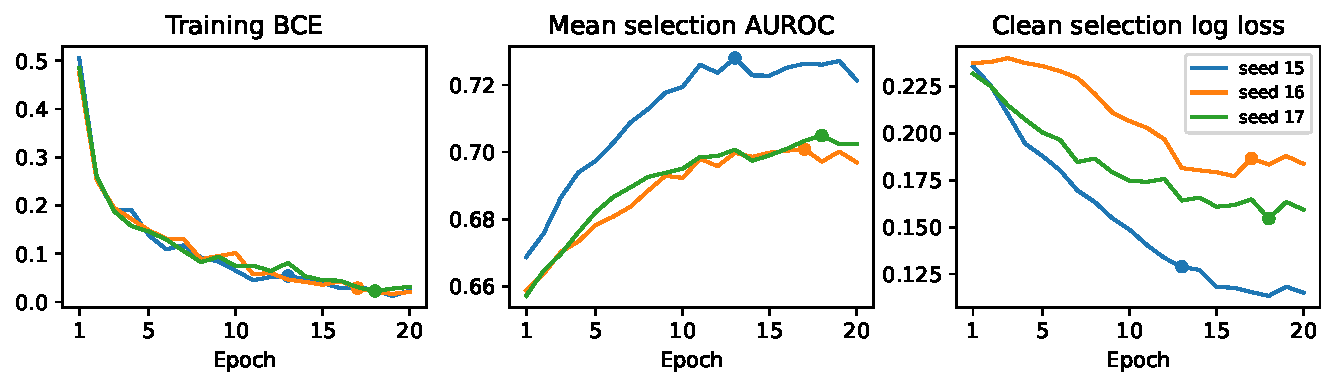
\includegraphics[width=\linewidth]{validation_training_curves.pdf}\end{center}
Optimization uses AdamW: adapter learning rate $10^{-4}$, temporary-head learning rate $10^{-3}$, weight decay 0.01 and gradient clipping 1. The same 1,056 clean rows fit weights in every epoch. Dots mark the retained epoch for each seed. The training loss is the temporary head's weighted BCE; selection AUROC and clean log loss use a freshly fitted training-only logistic probe at each epoch.

\begin{center}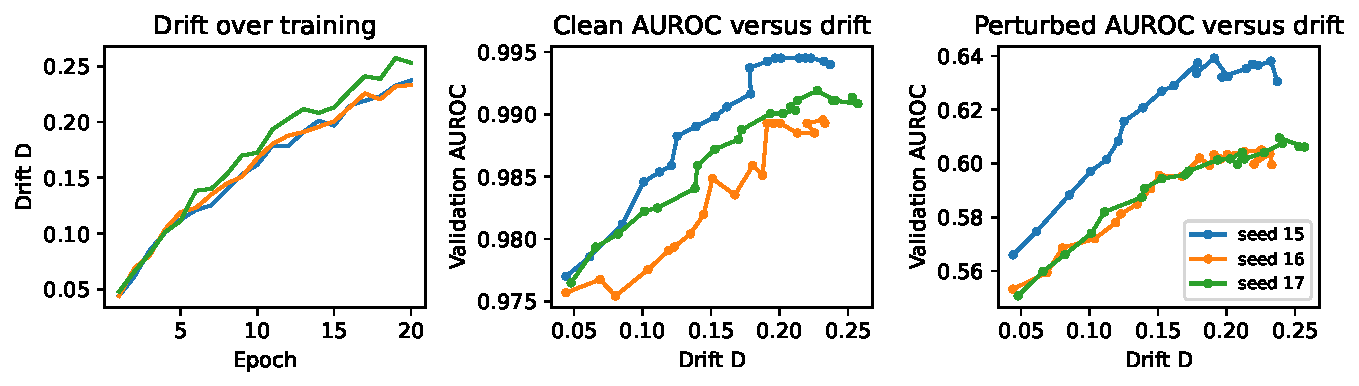
\includegraphics[width=\linewidth]{drift_training_curves.pdf}\end{center}
Drift is measured on the same 132 clean selection texts at each epoch, relative to their frozen representations. The third panel averages zero-width, homoglyph and base64 validation AUROCs. Curves describe association during training; they do not establish that drift causes detection gains.
\clearpage
\section*{Appendix D: concept robustness details}
\begin{center}\resizebox{\linewidth}{!}{\begin{tabular}{lrlll}
\toprule
Method & Seed & Zero-width & Homoglyph & Base64\\\midrule
frozen & 15 & -0.0665 [-0.2789, 0.3098] & 0.2213 [-0.2468, 0.5374] & 0.0294 [-0.3205, 0.3534]\\
lora & 15 & -0.0269 [-0.2860, 0.2494] & 0.0911 [-0.2299, 0.4509] & -0.0408 [-0.3332, 0.2225]\\
lora & 16 & -0.0429 [-0.3391, 0.2605] & 0.1603 [-0.2200, 0.5507] & -0.0133 [-0.3662, 0.2744]\\
lora & 17 & -0.0321 [-0.3057, 0.2525] & 0.2100 [-0.1588, 0.5673] & -0.0771 [-0.3462, 0.2070]\\
\bottomrule\end{tabular}
}\end{center}
Initial single 20-pair draw: clean/perturbed cosine and 95\% stratified class-bootstrap interval. This sample is not representative of the repeated-sampling results in Appendix E.

\code{random\_concept\_pairs.csv} records the 20 fixed test pairs and both source IDs. \code{random\_concept\_perturbations.csv} contains their 160 texts (40 sources across four conditions); \code{random\_concept\_robustness.csv} stores the measured similarities and bootstrap intervals. No prompt is reused within either sampled class. There is no topic matching or semantic acceptance filter, so this broad label contrast can include publisher-label ambiguity and class-correlated shortcuts. Bootstrap intervals condition on the trained models and available sampled sources; they do not resolve those semantic limitations.
\begin{center}\small\begin{tabular}{rlll}
\toprule
LoRA seed & Perturbation & $R_m-R_0$ & Paired 95\% interval\\\midrule
15 & zero\_width & +0.0397 & [-0.2854, +0.2987]\\
15 & homoglyph & -0.1302 & [-0.2899, +0.1994]\\
15 & base64 & -0.0701 & [-0.3077, +0.2814]\\
16 & zero\_width & +0.0236 & [-0.3512, +0.3269]\\
16 & homoglyph & -0.0610 & [-0.3218, +0.3107]\\
16 & base64 & -0.0427 & [-0.3736, +0.3727]\\
17 & zero\_width & +0.0344 & [-0.3504, +0.3229]\\
17 & homoglyph & -0.0113 & [-0.2880, +0.3508]\\
17 & base64 & -0.1064 & [-0.3924, +0.3226]\\
\bottomrule\end{tabular}
\end{center}
$R_m(T)-R_0(T)$ uses the same resampled source IDs across models and conditions, while resampling the two unmatched classes independently within dataset. Intervals spanning zero leave the direction of the change uncertain.

\textbf{Earlier quoted-control diagnostics (different concept).} The earlier analysis screened 24 training and 24 test injection sources (seed 17, at most 80 whitespace words). Controls quote the same source as inert data and request analysis without execution, using different training/test wrapper templates. GPT screened override intent and benign-control intent; \ConceptTrainCount{} training and \ConceptTestCount{} test pairs passed. These are automatically screened rather than independently human-verified pairs and are separate from the new 20 random label pairs.
\begin{center}\resizebox{\linewidth}{!}{\begin{tabular}{lrllll}
\toprule
Method & Seed & Clean gap & Homoglyph gap & Clean contrast cosine & Homoglyph contrast cosine\\
\midrule
frozen & 15 & 3.168 & 1.106 & 0.362 & 0.182\\
lora & 15 & 3.221 & 1.151 & 0.342 & 0.188\\
lora & 16 & 3.341 & 1.193 & 0.355 & 0.194\\
lora & 17 & 3.060 & 1.143 & 0.338 & 0.188\\
\bottomrule\end{tabular}
}\end{center}
The earlier held-out projected gap is $M_m=N^{-1}\sum_i u_m^\top[h_m(I_i)-h_m(B_i)]$, both clean and with homoglyph substitution applied to both members. The clean training-estimated $u_m$ stays fixed. Contrast cosine is the mean cosine between each held-out pair difference and $u_m$. These values do not measure the new random-sample direction stability $R_m(T)$.

The attached paper suggestion by Dr. Verma, \href{https://arxiv.org/abs/2508.11667}{GPS}, motivates examining embedding sensitivity; it does not make direction stability a semantic guarantee.

\clearpage
\section*{Appendix E: concept sample-size sensitivity}
\textbf{Sampling procedure and code.} The fully executed \code{concept\_sample\_size.ipynb} uses cached representations only. Its first code cell sets \code{SAMPLE\_SEEDS = range(17, 117)} and constructs the subsets; the second computes concept vectors and checks the original 20-pair result; the third summarizes draws and matched model changes; the fourth plots them.
\begin{enumerate}
\setlength{\itemsep}{0pt}\setlength{\parsep}{0pt}\setlength{\topsep}{2pt}
\item Form four test pools: deepset injection (60), deepset benign (56), Safe-Guard injection (63), and Safe-Guard benign (136). For each seed 17--116, initialize \code{np.random.default\_rng(seed)} and independently shuffle each pool with \code{rng.permutation}.
\item At each $K\in\{10,20,40,60,80,100,112\}$, take the first $K/2$ entries from each shuffled pool. Thus $K=20$ selects 10 from each pool: 20 injections and 20 benign prompts. Sampling is without replacement within a subset; prompts can recur across seeds. Larger sizes extend the same shuffled prefixes, producing nested samples.
\item Reuse those source IDs for frozen and all three LoRA models, and for clean and perturbed conditions. Compute separate clean/perturbed concept vectors and their cosine for each draw. No encoder inference or model fitting is repeated.
\item Average the 100 resulting cosines separately for each model, training seed, size and perturbation. Compute sampling SD and 5th--95th percentiles from those 100 cosines, and match the same subset when taking LoRA-minus-frozen differences. Training seeds 15/16/17 remain separate; the subsets are not independent test datasets or additional training runs.
\end{enumerate}
From \code{metrics\_export/}, run on CPU with \texttt{jupyter execute --inplace --timeout=600 concept\_sample\_size.ipynb}.
\begin{center}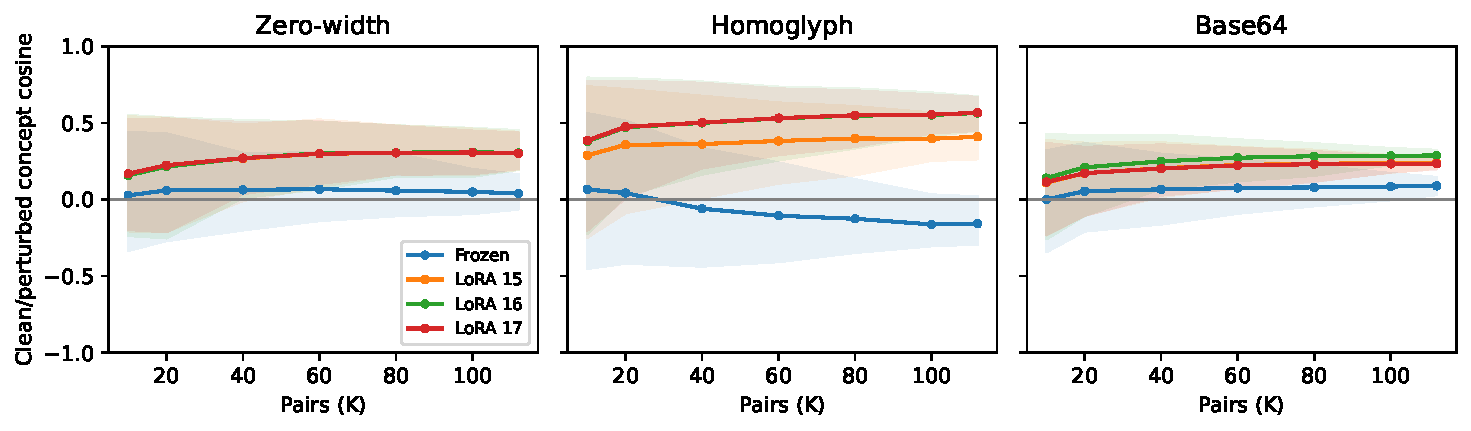
\includegraphics[width=\linewidth]{concept_sample_size_stability.pdf}\end{center}
Lines show the mean of the 100 per-draw cosines; bands show their 5th--95th percentiles. These are finite-pool sampling spreads, not population confidence intervals. The original fixed 20-pair draw used direct sampling rather than nested permutation prefixes; its values are independently reproduced by this notebook.
\begin{center}\footnotesize\begin{tabular}{rlll}
\toprule
Pairs $K$ & Perturbation & Frozen mean $R$ & LoRA mean $R$ range across seeds\\\midrule
10 & zero\_width & 0.0269 & 0.1572--0.1679\\
10 & homoglyph & 0.0656 & 0.2876--0.3852\\
10 & base64 & 0.0001 & 0.1092--0.1393\\
20 & zero\_width & 0.0591 & 0.2144--0.2238\\
20 & homoglyph & 0.0420 & 0.3567--0.4741\\
20 & base64 & 0.0542 & 0.1713--0.2098\\
40 & zero\_width & 0.0629 & 0.2679--0.2698\\
40 & homoglyph & -0.0603 & 0.3616--0.5013\\
40 & base64 & 0.0664 & 0.2021--0.2489\\
60 & zero\_width & 0.0672 & 0.2985--0.3012\\
60 & homoglyph & -0.1057 & 0.3818--0.5306\\
60 & base64 & 0.0752 & 0.2221--0.2724\\
80 & zero\_width & 0.0578 & 0.3037--0.3056\\
80 & homoglyph & -0.1258 & 0.3979--0.5495\\
80 & base64 & 0.0789 & 0.2303--0.2823\\
100 & zero\_width & 0.0495 & 0.3059--0.3083\\
100 & homoglyph & -0.1627 & 0.3962--0.5538\\
100 & base64 & 0.0845 & 0.2324--0.2850\\
112 & zero\_width & 0.0399 & 0.3001--0.3036\\
112 & homoglyph & -0.1579 & 0.4090--0.5655\\
112 & base64 & 0.0887 & 0.2340--0.2873\\
\bottomrule\end{tabular}
\end{center}
Table ranges span the three LoRA seeds' means over 100 subsets. At 112 pairs, all 100 matched changes are positive for every condition and seed. Full-pool references use all 315 prompts with equal dataset weights. These results support relative stability within this pool, without establishing semantic purity or complete invariance.

The CSV outputs listed in README contain per-draw cosines, Euclidean distances, convergence to full-pool directions and matched model changes. Unit Euclidean distance mirrors cosine. Base64 alignment improves without reliable detection, so direction stability is not sufficient for operational robustness.
\end{document}
